
- axisymmetric case only

As seen in stone~\ref{f151}, there are (at least) two ways to compute the normal at the
nodes on the surface: $\vec{n}_1$ which is purely geometric and $\vec{n}_2$ which is based 
on an integration of the basis function derivatives.
We found that in the case of the annulus the two coincided to machine precision. 
Let us now turn the half annulus. As an experiment, {\it all} nodes on the hull are flagged
and the normal $\vec{n}_2$ is computed. 
Since this normal is a function of basis functions and requires an integration 
over elements, we can ask ourselves whether the mapping and/or the number
of quadrature points influence the results of the normal calculations.
The {\tt script\_normals} bash script runs the required models - note that the
$Q_1$ mapping and nqperdim=2 have been removed from the loops.

\begin{center}
\includegraphics[width=8cm]{RESULTS/normals/nx}
\includegraphics[width=8cm]{RESULTS/normals/ny}\\
\includegraphics[width=8cm]{RESULTS/normals/nnx}
\includegraphics[width=8cm]{RESULTS/normals/nny}\\
{\captionfont components of the normal vector on the hull (first line),
on the surface (second line). Mesh is 8x96.}
\end{center}

We find that these normal vector components do not seem to depend on the mapping nor quadrature,
and that on the curved parts they match their geometrical counterparts $\vec{n}_1$.
These normal vectors are shown here:

\begin{center}
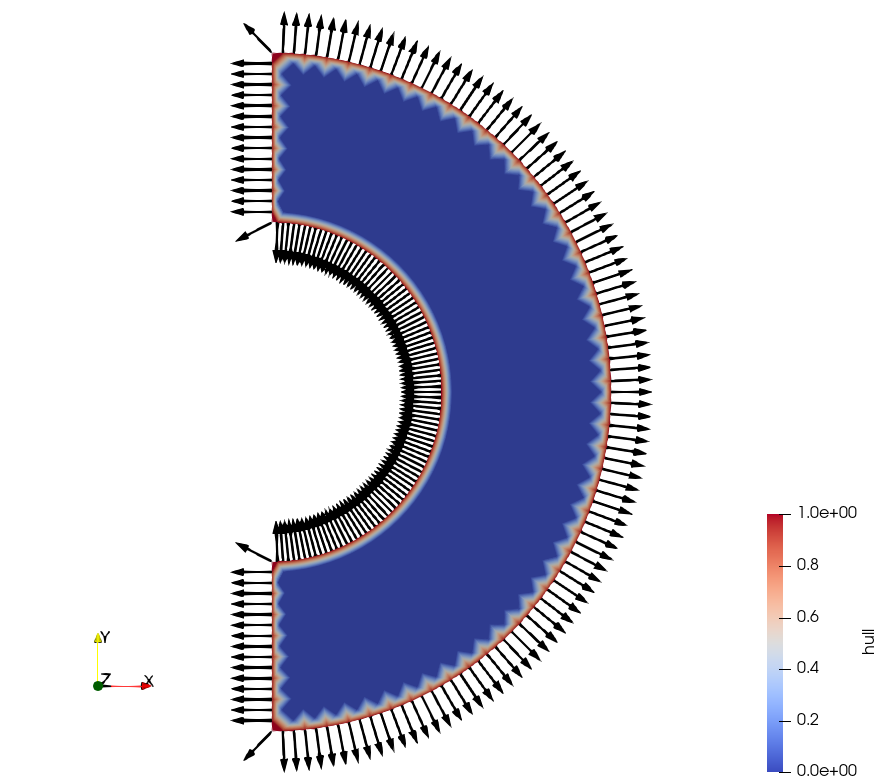
\includegraphics[width=6cm]{RESULTS/normals/normals}
\end{center}

Obviously, we need to look closer at the four nodes that belong to the surface and the cmb with $x=0$.
On the one hand they belong the vertical boundary $x=0$ so their horizontal velocity component should be zero (axisymmetry).
On the other hand they also belong to the curved boundaries. In the case of a near infinite resolution the 
normal to the curved part would align with the vertical axis so that we would then have $v=0$. 
In the end these 4 points should be prescribed no-slip boundary conditions.

In our case here only the surface can be prescribed free slip boundary conditions and there are {\python nnt} points at the surface.
Removing the 2 extremities, we have {\python nnt-2} Lagrange multipliers. Note that then how we compute normals is not relevant.

\begin{center}
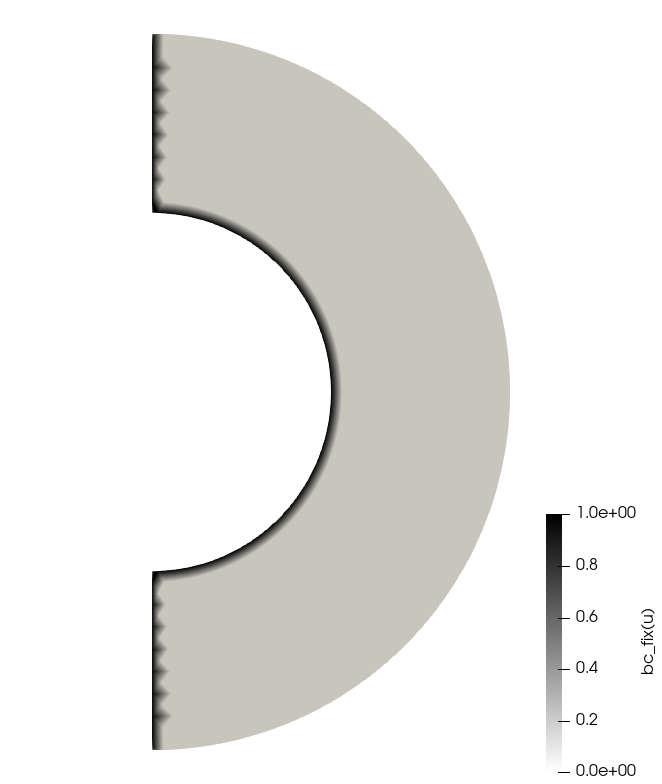
\includegraphics[width=6cm]{images/bcfix_u}
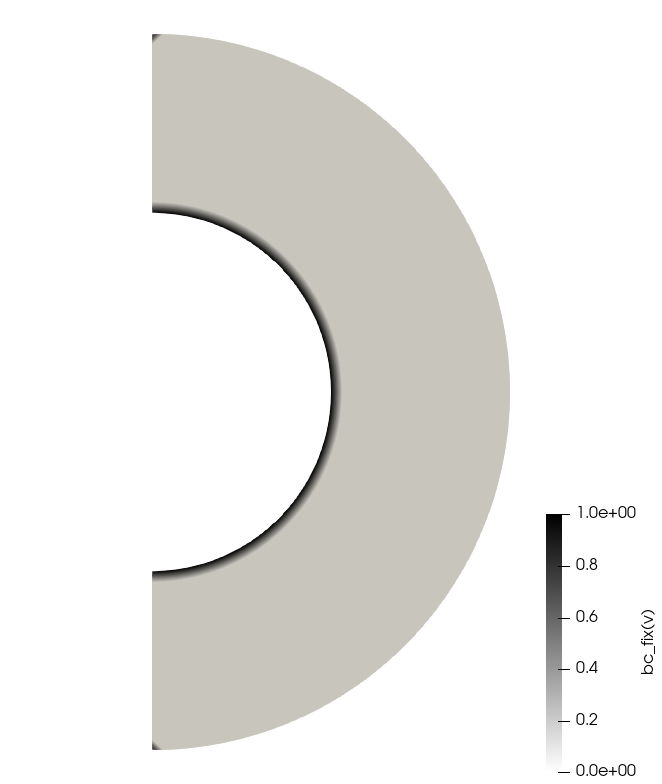
\includegraphics[width=6cm]{images/bcfix_v}\\
{\captionfont horizontal and vertical boundary condition indicators.}
\end{center}


